\documentclass[12pt]{article}

\usepackage{tikz}
\usepackage{tikz-uml}
\usetikzlibrary{circuits.logic.IEC}
\usetikzlibrary{circuits.logic.US}


\begin{document}



\begin{figure}
\begin{tikzpicture}
\draw (0,0) --(1,2);
\end{tikzpicture}
\caption{Do not forget!
Make it explicit enough that readers
can figure out what you are doing.}
\end{figure}

.\newline

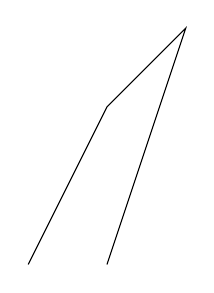
\begin{tikzpicture}
\draw (0,0) --(1,2) -- (2,3) -- (1,0);
\end{tikzpicture}

.\newline

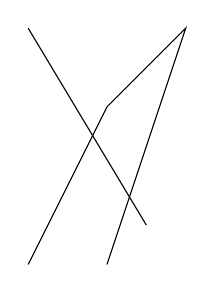
\begin{tikzpicture}
\draw (0,0) --(1,2) -- (2,3) -- (1,0);
\draw (0,3) -- (1.5,0.5);
\end{tikzpicture}


.\newline


\begin{tikzpicture}[scale=3]
\draw (0,0) -- (1,1);
\end{tikzpicture}


.\newline

\begin{tikzpicture}[xscale=3]
\draw (0,0) -- (1,1);
\end{tikzpicture}



.\newline


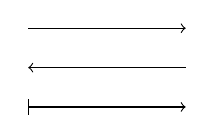
\begin{tikzpicture}
\draw [->] (0,0) -- (2,0);
\draw [<-] (0, -0.5) -- (2,-0.5);
\draw [|->] (0,-1) -- (2,-1);
\end{tikzpicture}

.\newline


\begin{tikzpicture}
\draw [<->] (0,2) -- (0,0) -- (3,0);
\end{tikzpicture}


.\newline

\begin{tikzpicture}
\draw [->] (0,0) -- (0,2) ;
\draw [->] (0,0) -- (3,0);
\end{tikzpicture}


.\newline


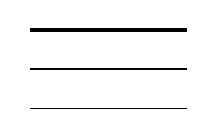
\begin{tikzpicture}
\draw [ultra thick] (0,1) -- (2,1);
\draw [thick] (0,0.5) -- (2,0.5);
\draw [thin] (0,0) -- (2,0);
\end{tikzpicture}


.\newline

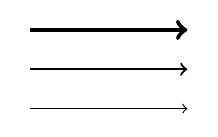
\begin{tikzpicture}
\draw [ultra thick,->] (0,1) -- (2,1);
\draw [thick,->] (0,0.5) -- (2,0.5);
\draw [thin,->] (0,0) -- (2,0);
\end{tikzpicture}


.\newline


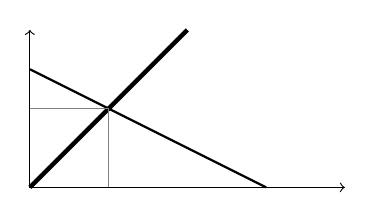
\begin{tikzpicture}
\draw [<->] (0,2) -- (0,0) -- (4,0);
\draw [thick] (0,1.5) -- (3,0);
\draw [ultra thick] (0,0) -- (2,2);
\draw [help lines] (1,0) -- (1,1) -- (0,1);
\end{tikzpicture}

.\newline


\begin{tikzpicture}
\draw [line width=12] (0,0) -- (2,0);
\draw [line width=0.2cm] (4,.75) -- (5,.25);
\end{tikzpicture}

.\newline


\begin{tikzpicture}
\draw [dashed, ultra thick] (0,1) -- (2,1);
\draw [dashed] (0, 0.5) -- (2,0.5);
\draw [dotted] (0,0) -- (2,0);
\end{tikzpicture}


.\newline




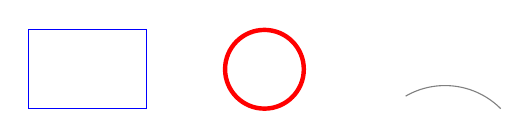
\begin{tikzpicture}
\draw [blue] (0,0) rectangle (1.5,1);
\draw [red, ultra thick] (3,0.5) circle [radius=0.5];;
\draw [gray] (6,0) arc [radius=1, start angle=45, end angle= 120];
\end{tikzpicture}




.\newline




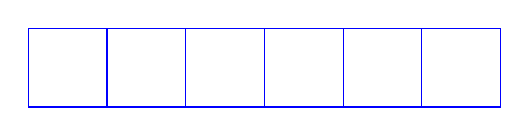
\begin{tikzpicture}
\foreach \x in {0,1,2,3,4,5}
	\draw [blue] (\x,0) rectangle (\x+1,1);
\end{tikzpicture}




.\newline



\begin{center}
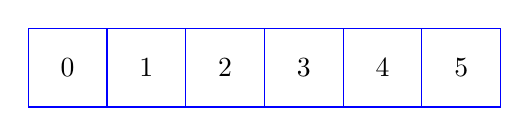
\begin{tikzpicture}
\foreach \x in {0,1,2,3,4,5} {
	\draw [blue] (\x,0) rectangle (\x+1,1); 
	\draw (\x+.5,.5) node {\x}; 
}
\end{tikzpicture}
\end{center}


.\newline
.\newline



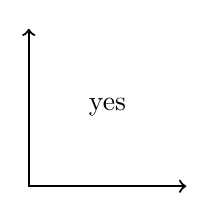
\begin{tikzpicture}
\draw [thick, <->] (0,2) -- (0,0) -- (2,0);
\node at (1,1) {yes};
\end{tikzpicture}

.\newline
.\newline


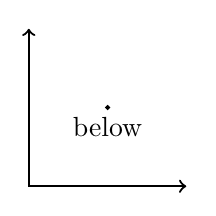
\begin{tikzpicture}
\draw [thick, <->] (0,2) -- (0,0) -- (2,0);
\draw[fill] (1,1) circle [radius=0.025];
\node [below] at (1,1) {below};
\end{tikzpicture}


.\newline
.\newline



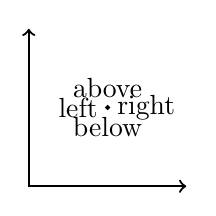
\begin{tikzpicture}
\draw [thick, <->] (0,2) -- (0,0) -- (2,0);
\draw[fill] (1,1) circle [radius=0.025];
\node [below] at (1,1) {below};
\node [above] at (1,1) {above};
\node [left] at (1,1) {left};
\node [right] at (1,1) {right};
\end{tikzpicture}



.\newline
.\newline





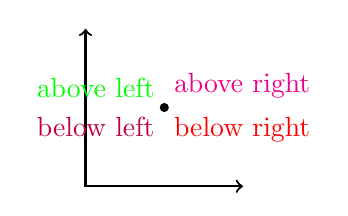
\begin{tikzpicture}[scale=2]
\draw [thick, <->] (0,1) -- (0,0) -- (1,0);
\draw[fill] (.5,.5) circle [radius=0.025];
\node [below right, red] at (.5,.5) {below right};
\node [above left, green] at (.5,.5) {above left};
\node [below left, purple] at (.5,.5) {below left};
\node [above right, magenta] at (.5,.5) {above right};
\end{tikzpicture}



.\newline
.\newline




\begin{tikzpicture}[xscale=3, yscale=1.5]
\draw [thick, <->] (0,1) -- (0,0) -- (1,0);
\node [below right] at (1,0) {$x$};
\node [left] at (0,1) {$y$};
\draw[fill] (.4,.6) circle [radius=.5pt];
\node[above right] (.4,.6) {$A$};
\end{tikzpicture}




.\newline
.\newline




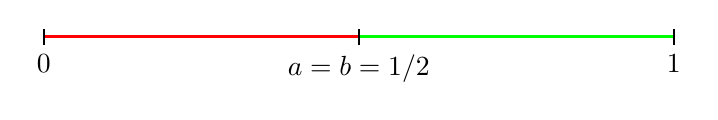
\begin{tikzpicture}[xscale=8]
\draw[-][draw=red, very thick] (0,0) -- (.5,0);
\draw[-][draw=green, very thick] (.5,0) -- (1,0);
\draw [thick] (0,-.1) node[below]{0} -- (0,0.1);
\draw [thick] (0.5,-.1) node[below]{$a=b=1/2$} -- (0.5,0.1);
\draw [thick] (1,-.1) node[below]{1} -- (1,0.1);
\end{tikzpicture}


.\newline
.\newline

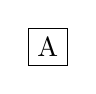
\begin{tikzpicture}
\node [draw] (and1) at (0,0) {A};
\end{tikzpicture}

.\newline
.\newline


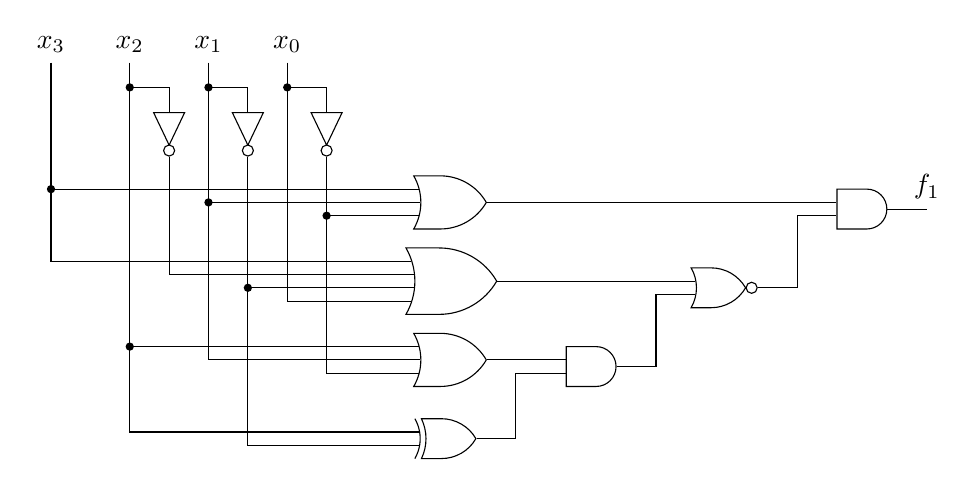
\begin{tikzpicture}[label distance=2mm]
\tikzstyle{branch}=[fill,shape=circle,minimum size=3pt,inner sep=0pt]
    \node (x3) at (0,0) {$x_3$};
    \node (x2) at (1,0) {$x_2$};
    \node (x1) at (2,0) {$x_1$};
    \node (x0) at (3,0) {$x_0$};

    \node[not gate US, draw, rotate=-90] at ($(x2)+(0.5,-1)$) (Not2) {};
    \node[not gate US, draw, rotate=-90] at ($(x1)+(0.5,-1)$) (Not1) {};
    \node[not gate US, draw, rotate=-90] at ($(x0)+(0.5,-1)$) (Not0) {};

    \node[or gate US, draw, logic gate inputs=nnn] at ($(x0)+(2,-2)$) (Or1) {};
    \node[or gate US, draw, logic gate inputs=nnnn] at ($(Or1)+(0,-1)$) (Or2) {};
    \node[or gate US, draw, logic gate inputs=nnn] at ($(Or2)+(0,-1)$) (Or3) {};
    \node[xor gate US, draw, logic gate inputs=nn] at ($(Or3)+(0,-1)$) (Xor1) {};
    
    \node[and gate US, draw, logic gate inputs=nn, anchor=input 1] at ($(Or3.output)+(1,0)$) (And1) {};
    \node[nor gate US, draw, logic gate inputs=nn, anchor=input 1] at ($(Or2.output -| And1.output)+(1,0)$) (Nor1) {};
    \node[and gate US, draw, logic gate inputs=nn, anchor=input 1] at ($(Or1.output -| Nor1.output)+(1,0)$) (And2) {};

    \foreach \i in {2,1,0}
    {
        \path (x\i) -- coordinate (punt\i) (x\i |- Not\i.input);
        \draw (punt\i) node[branch] {} -| (Not\i.input);
    }
    \draw (x3) |- (Or2.input 1);
    \draw (x3 |- Or1.input 1) node[branch] {} -- (Or1.input 1);
    \draw (x2) |- (Xor1.input 1);
    \draw (x2 |- Or3.input 1) node[branch] {} -- (Or3.input 1);
    \draw (Not2.output) |- (Or2.input 2);
    \draw (x1) |- (Or3.input 2);
    \draw (x1 |- Or1.input 2) node[branch] {} -- (Or1.input 2);
    \draw (Not1.output) |- (Xor1.input 2);
    \draw (Not1.output |- Or2.input 3) node[branch] {} -- (Or2.input 3);
    \draw (x0) |- (Or2.input 4);
    \draw (Not0.output) |- (Or3.input 3);
    \draw (Not0.output |- Or1.input 3) node[branch] {} -- (Or1.input 3);
    \draw (Or3.output) -- (And1.input 1);
    \draw (Xor1.output) -- ([xshift=0.5cm]Xor1.output) |- (And1.input 2);
    \draw (Or2.output) -- (Nor1.input 1);
    \draw (And1.output) -- ([xshift=0.5cm]And1.output) |- (Nor1.input 2);
    \draw (Or1.output) -- (And2.input 1);
    \draw (Nor1.output) -- ([xshift=0.5cm]Nor1.output) |- (And2.input 2);
    \draw (And2.output) -- ([xshift=0.5cm]And2.output) node[above] {$f_1$};

\end{tikzpicture}






.\newline
.\newline


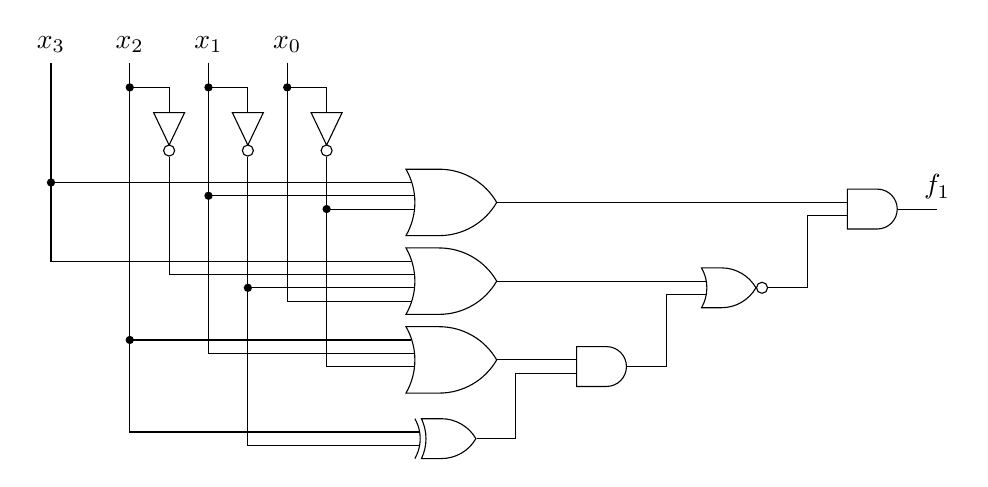
\begin{tikzpicture}[label distance=2mm]
\tikzstyle{branch}=[fill,shape=circle,minimum size=3pt,inner sep=0pt]
    \node (x3) at (0,0) {$x_3$};
    \node (x2) at (1,0) {$x_2$};
    \node (x1) at (2,0) {$x_1$};
    \node (x0) at (3,0) {$x_0$};

    \node[not gate US, draw, rotate=-90] at ($(x2)+(0.5,-1)$) (Not2) {};
    \node[not gate US, draw, rotate=-90] at ($(x1)+(0.5,-1)$) (Not1) {};
    \node[not gate US, draw, rotate=-90] at ($(x0)+(0.5,-1)$) (Not0) {};

    \node[or gate US, draw, logic gate inputs=nnnn] at ($(x0)+(2,-2)$) (Or1) {};
    \node[or gate US, draw, logic gate inputs=nnnn] at ($(Or1)+(0,-1)$) (Or2) {};
    \node[or gate US, draw, logic gate inputs=nnnn] at ($(Or2)+(0,-1)$) (Or3) {};
    \node[xor gate US, draw, logic gate inputs=nn] at ($(Or3)+(0,-1)$) (Xor1) {};
    
    \node[and gate US, draw, logic gate inputs=nn, anchor=input 1] at ($(Or3.output)+(1,0)$) (And1) {};
    \node[nor gate US, draw, logic gate inputs=nn, anchor=input 1] at ($(Or2.output -| And1.output)+(1,0)$) (Nor1) {};
    \node[and gate US, draw, logic gate inputs=nn, anchor=input 1] at ($(Or1.output -| Nor1.output)+(1,0)$) (And2) {};
	
	% this foreach is for drawing 
	% from x0,x1,x2 to not gates
	% x\i means x0, x1 , x2
    \foreach \i in {2,1,0}
    {
        \path (x\i) -- coordinate (punt\i) (x\i |- Not\i.input);
        \draw (punt\i) node[branch] {} -| (Not\i.input);
    }
    
    \draw (x3) |- (Or2.input 1);
    \draw (x3 |- Or1.input 1) node[branch] {} -- (Or1.input 1);
    \draw (x2) |- (Xor1.input 1);
    \draw (x2 |- Or3.input 1) node[branch] {} -- (Or3.input 1);
    \draw (Not2.output) |- (Or2.input 2);
    \draw (x1) |- (Or3.input 2);
    \draw (x1 |- Or1.input 2) node[branch] {} -- (Or1.input 2);
    \draw (Not1.output) |- (Xor1.input 2);
    \draw (Not1.output |- Or2.input 3) node[branch] {} -- (Or2.input 3);
    \draw (x0) |- (Or2.input 4);
    \draw (Not0.output) |- (Or3.input 3);
    \draw (Not0.output |- Or1.input 3) node[branch] {} -- (Or1.input 3);
    \draw (Or3.output) -- (And1.input 1);
    \draw (Xor1.output) -- ([xshift=0.5cm]Xor1.output) |- (And1.input 2);
    \draw (Or2.output) -- (Nor1.input 1);
    \draw (And1.output) -- ([xshift=0.5cm]And1.output) |- (Nor1.input 2);
    \draw (Or1.output) -- (And2.input 1);
    \draw (Nor1.output) -- ([xshift=0.5cm]Nor1.output) |- (And2.input 2);
    \draw (And2.output) -- ([xshift=0.5cm]And2.output) node[above] {$f_1$};

\end{tikzpicture}






.\newline
.\newline





\begin{tikzpicture}
\node[not gate US, draw] at (0,0) (Not1) {};
\node[or gate US, draw, logic gate inputs=nn] at (0,-2) (Or1) {};
\node[or gate US, draw, logic gate inputs=nnn] at (0,-4) (Or2) {};
\node[or gate US, draw, logic gate inputs=nnnn] at (0,-6) (Or3) {};

\draw (-1,0) -- (Not1.input) ;
\draw (Not1.output) -- ($(Not1.output)+(1,0)$);

\draw ($(Or1.input 1)+(-1,0)$) -- (Or1.input 1) ;
\draw ($(Or1.input 2)+(-1,0)$) -- (Or1.input 2) ;
\draw (Or1.output) -- ($(Or1.output)+(1,0)$);


\draw ($(Or2.input 1)+(-1,0)$) node[left] {$x_{1}$} -- (Or2.input 1) ;
%\draw ($(Or2.input 2)+(-1,0)$) node[left] {$x_{2}$} -- (Or2.input 2) ;
\draw ($(Or2.input 3)+(-1,0)$) node[left] {$x_{3}$} -- (Or2.input 3) ;
\draw (Or2.output) -- ($(Or2.output)+(1,0)$) node[right] {$f$};


\draw ($(Or3.input 1)+(-1,0)$) -- (Or3.input 1) ;
\draw ($(Or3.input 2)+(-1,0)$) -- (Or3.input 2) ;
\draw ($(Or3.input 3)+(-1,0)$) -- (Or3.input 3) ;
\draw ($(Or3.input 4)+(-1,0)$) -- (Or3.input 4) ;
\draw (Or3.output) -- ($(Or3.output)+(1,0)$);
\end{tikzpicture}






.\newline
.\newline





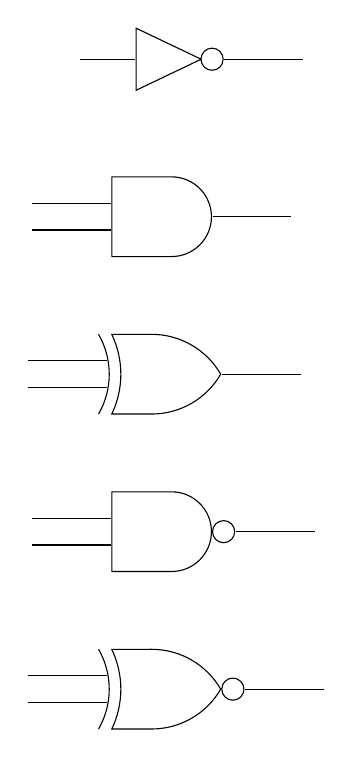
\begin{tikzpicture}
\node[not gate US, draw,scale=2] at (0,0) (Not1) {};
\node[and gate US, draw, logic gate inputs=nn,scale=2] at (0,-2) (and1) {};
\node[xor gate US, draw, logic gate inputs=nn,scale=2] at (0,-4) (xor1) {};
\node[nand gate US, draw, logic gate inputs=nn,scale=2] at (0,-6) (nand1) {};
\node[xnor gate US, draw, logic gate inputs=nn,scale=2] at (0,-8) (xnor1) {};

\draw (-1,0) -- (Not1.input) ;
\draw (Not1.output) -- ($(Not1.output)+(1,0)$);

\draw ($(and1.input 1)+(-1,0)$) -- (and1.input 1) ;
\draw ($(and1.input 2)+(-1,0)$) -- (and1.input 2) ;
\draw (and1.output) -- ($(and1.output)+(1,0)$);


\draw ($(xor1.input 1)+(-1,0)$) -- (xor1.input 1) ;
\draw ($(xor1.input 2)+(-1,0)$) -- (xor1.input 2) ;
\draw (xor1.output) -- ($(xor1.output)+(1,0)$);


\draw ($(nand1.input 1)+(-1,0)$) -- (nand1.input 1) ;
\draw ($(nand1.input 2)+(-1,0)$) -- (nand1.input 2) ;
\draw (nand1.output) -- ($(nand1.output)+(1,0)$);


\draw ($(xnor1.input 1)+(-1,0)$) -- (xnor1.input 1) ;
\draw ($(xnor1.input 2)+(-1,0)$) -- (xnor1.input 2) ;
\draw (xnor1.output) -- ($(xnor1.output)+(1,0)$);
\end{tikzpicture}







.\newline
.\newline





\begin{tikzpicture}
\node[not gate US, draw,scale=2] at (0,0) (Not1) {};
\node[and gate US, draw, logic gate inputs=nn,scale=2] at (0,-2) (and1) {};
\node[xor gate US, draw, logic gate inputs=nn,scale=2] at (3,-1) (xor1) {};


\draw (-1,0) -- (Not1.input) ;
\draw (Not1.output) -- ($(Not1.output)+(.9,0)$) |- (xor1.input 1);

\draw ($(and1.input 1)+(-1,0)$) -- (and1.input 1) ;
\draw ($(and1.input 2)+(-1,0)$) -- (and1.input 2) ;
\draw (and1.output) -- ($(and1.output)+(1,0)$) |- (xor1.input 2);


\draw (xor1.output) -- ($(xor1.output)+(1,0)$);

\end{tikzpicture}



.\newline
.\newline



\begin{tikzpicture}
\node[not gate US, draw,scale=2] at (0,0) (Not1) {};
\node[and gate US, draw, logic gate inputs=nn,scale=2] at (0,-2) (and1) {};
\node[xor gate US, draw, logic gate inputs=nn,scale=2] at (3,-1) (xor1) {};
\node[nand gate US, draw, logic gate inputs=nn,scale=2] at (6,-2) (nand1) {};

\draw (-1,0) -- (Not1.input) ;
\draw (Not1.output) -- ($(Not1.output)+(.9,0)$) |- (xor1.input 1);

\draw ($(and1.input 1)+(-1,0)$) -- (and1.input 1) ;
\draw ($(and1.input 2)+(-1,0)$) -- (and1.input 2) ;
\draw (and1.output) -- ($(and1.output)+(1,0)$) |- (xor1.input 2);


%\draw (xor1.output) -- ($(xor1.output)+(1,0)$);
\draw (xor1.output) -- ($(xor1.output)+(1,0)$)  |- (nand1.input 1);
\draw (0,-3) -- (5,-3) |- (nand1.input 2);

\end{tikzpicture}




.\newline
.\newline




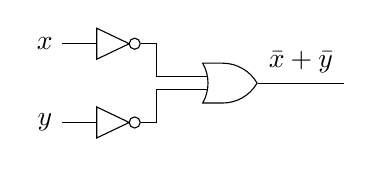
\begin{tikzpicture}
    \node (x) at (0, 1) {$x$};
    \node (y) at (0, 0) {$y$};

    \node[not gate US, draw] at ($(x) + (0.8, 0)$) (notx) {};
    \node[not gate US, draw] at ($(y) + (0.8, 0)$) (noty) {};
    \node[or gate US, draw, rotate=0, logic gate inputs=nn] at ($(noty) + (1.5, 0.5)$) (xory) {};

    \draw (x) -- (notx.input);
    \draw (y) -- (noty.input);

    \draw (notx.output) -- ([xshift=0.2cm]notx.output) |- (xory.input 1);
    \draw (noty.output) -- ([xshift=0.2cm]noty.output) |- (xory.input 2);

    \draw (xory.output) -- node[above]{$\bar x + \bar y$} ($(xory) + (1.5, 0)$);
\end{tikzpicture}



.\newline
.\newline





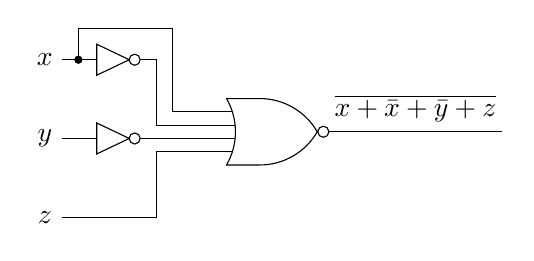
\begin{tikzpicture}
\tikzstyle{branch}=[fill, shape=circle, minimum size=3pt, inner sep=0pt]

    \node (x) at (0, 2) {$x$};
    \node (y) at (0, 1) {$y$};
    \node (z) at (0, 0) {$z$};

    \node[not gate US, draw] at ($(x) + (0.8, 0)$) (notx) {};
    \node[not gate US, draw] at ($(y) + (0.8, 0)$) (noty) {};
    \node[nor gate US, draw, rotate=0, logic gate inputs=nnnn] at ($(noty) + (2, 0.085)$) (xory) {};

    \draw (x) -- (notx.input);
    \draw (y) -- (noty.input);

    \path ($(notx.input) + (0.2, 0)$) -- coordinate (puntx) (x |- notx);
    \draw (x) -- (puntx) node[branch] {} |- ($(notx.output) + (0.4, 0.4)$) |- (xory.input 1);

    \draw (notx.output) -- ([xshift=0.2cm]notx.output) |- (xory.input 2);
    \draw (noty.output) -- ([xshift=0.2cm]noty.output) |- (xory.input 3);
    \draw (z) -| ($(noty.output) + (0.2, -0.5)$) |- (xory.input 4);

    \draw (xory.output) -- node[above]{$\overline{x + \bar x + \bar y + z}$} ($(xory) + (3, 0)$);
\end{tikzpicture}






\end{document}